\documentclass[11pt]{article}
\usepackage{amsmath, amssymb}
\usepackage{geometry}
\usepackage{hyperref}
\usepackage{graphicx}
\geometry{margin=2.5cm}

\newcommand{\ket}[1]{|#1\rangle}
\newcommand{\bra}[1]{\langle#1|}

\title{Block 3: Measuring Topology via Quantum Circuits}
\author{Seminar notes}
\date{\today}

\begin{document}
\maketitle

\section{Introduction}
In Block 2, we mapped the fermionic Kitaev chain to a system of qubits using the Jordan-Wigner transform. The resulting Hamiltonian is a 1D transverse-field XY model:
\begin{equation}
  H = -\frac{\mu}{2} \sum_{j=0}^{L-1} Z_j 
      + \frac{t - \Delta}{2} \sum_{j=0}^{L-2} X_j X_{j+1} 
      + \frac{t + \Delta}{2} \sum_{j=0}^{L-2} Y_j Y_{j+1}.
\end{equation}
For Block 3, our goal is to simulate this system using a quantum circuit framework (Qiskit). This requires two main steps:
\begin{enumerate}
  \item \textbf{State Preparation:} Initializing the qubits into the many-body ground state $\ket{\Phi_0^{(+)}}$.
  \item \textbf{Measurement:} Evaluating local and non-local (string) observables to detect the topological phase.
\end{enumerate}

\section{Approaches to Ground State Preparation}
Preparing the exact ground state of a strongly correlated many-body system is generally hard, but the Kitaev chain is integrable (it maps to free fermions). We have a few distinct paths to prepare the state on a quantum computer.

\subsection{Approach 1: Exact Free-Fermion State Preparation (Algebraic)}
Since the system is non-interacting, its ground state is a Slater determinant. Any Slater determinant can be prepared exactly using a polynomial-depth quantum circuit.
\begin{itemize}
  \item \textbf{Method:} We diagonalize the real-space BdG matrix to find the Bogoliubov transformation matrix $W$. Using QR or SVD-like decompositions, $W$ can be factored into a sequence of nearest-neighbor Givens rotations.
  \item \textbf{Circuit:} These rotations map directly to two-qubit fermionic simulation gates (e.g., $XX+YY$ rotations, known as fSim gates).
  \item \textbf{Pros:} Prepares the state exactly with 100\% theoretical fidelity. Provides a perfect theoretical baseline.
  \item \textbf{Cons:} The circuit depth scales linearly with $L$ (or $L^2 / 2$ for full basis transforms), which can be deep for NISQ devices.
\end{itemize}

\subsection{Approach 2: Variational Quantum Eigensolver (VQE)}
VQE is a hybrid quantum-classical heuristic. We define a parameterized quantum circuit $U(\vec{\theta})$ (the ansatz), prepare the state $\ket{\psi(\vec{\theta})} = U(\vec{\theta})\ket{0}$, measure the energy $E(\vec{\theta}) = \bra{\psi} H \ket{\psi}$, and use a classical optimizer to minimize $E$.
\begin{itemize}
  \item \textbf{Method:} We can use a Hamiltonian Variational Ansatz (HVA), which applies alternating layers of $e^{-i \theta_1 Z_j}$, $e^{-i \theta_2 X_j X_{j+1}}$, and $e^{-i \theta_3 Y_j Y_{j+1}}$ gates.
  \item \textbf{Pros:} The circuits are typically very shallow and resilient to certain systematic errors, making this the standard approach for near-term (NISQ) hardware.
  \item \textbf{Cons:} It is an approximation. Finding the global minimum can be difficult (barren plateaus), and the resulting state has a fidelity strictly less than 1.
\end{itemize}

\subsection{Approach 3: Exact Diagonalization Vector Loading (StateVector)}
For small systems ($L \le 12$), we can simply diagonalize the $2^L \times 2^L$ qubit Hamiltonian classically to find the exact state vector, and then forcefully load this vector into the Qiskit simulator.
\begin{itemize}
  \item \textbf{Pros:} Trivial to implement using \texttt{qiskit.QuantumCircuit.initialize()}.
  \item \textbf{Cons:} Not a true quantum algorithm. The initialization gate compiles to an exponentially deep circuit, so it is useless for real hardware. It only serves as a classical simulation tool to verify observables.
\end{itemize}

\paragraph{Selected Path (Revised for Week 5):} Based on the Week 5 Execution Plan, we must strictly deprecate \textbf{Approach 3 (StateVector)} and exact diagonalization using dense matrices. The architecture must fully transition to gate-based quantum circuit simulation. We will implement \textbf{Approach 2 (VQE)} with a parameterized quantum circuit (PQC) using $RY$ and $CX/CZ$ gates. The state output must achieve a fidelity of $F > 0.99$ compared to the exact state for small systems ($L \le 8$) before proceeding to measurements.

\section{Measuring Observables}

Once the ground state $\ket{\Phi}$ is prepared, we must measure the signatures of topology.

\subsection{Edge Observables (Local)}
In the topological phase, Majorana zero modes are localized at the edges. At the sweet spot ($t = \Delta, \mu = 0$), the Hamiltonian reduces to $H = t \sum Y_j Y_{j+1}$, completely decoupling the boundary operators $X_0$ and $X_{L-1}$. 
Therefore, the edge Majorana modes are directly related to the local Pauli observables:
\begin{equation}
  \mathcal{O}_{\text{edge}, L} = X_0, \qquad \mathcal{O}_{\text{edge}, R} = X_{L-1}.
\end{equation}
When evaluating $\bra{\Phi_0} X_0 \ket{\Phi_0}$, however, we must be careful: the absolute ground state has a definite parity, and a single $X$ operator flips parity. To observe the mode, we instead look at correlations or state transfers.

\subsection{String Order Parameters (Non-Local)}
The defining feature of a 1D topological phase is that it cannot be characterized by a local order parameter (like magnetization). Instead, it possesses hidden long-range order, detectable via a \textbf{String Order Parameter (SOP)}.
For the Kitaev chain mapped to qubits, the topological phase corresponds to the ferromagnetic phase of the transverse-field Ising/XY model. The appropriate string order parameter spanning sites $i$ and $j$ is:
\begin{equation}
  \text{SOP}(|i - j|) = \langle X_i \left( \prod_{k=i+1}^{j-1} Z_k \right) X_j \rangle.
\end{equation}
In the trivial phase ($|\mu| > 2t$), this expectation value decays exponentially to 0. 
In the topological phase ($|\mu| < 2t$), this string correlation attains a non-zero long-range asymptotic value as $|i-j| \to \infty$. 

\subsection{Shot-Based Sampling Requirement}
Analytical expectation values from statevectors must be discarded. The measurement protocol must execute shot-based sampling (e.g., \texttt{shots=8192}). 
\begin{itemize}
  \item \textbf{Local $\langle X_0 \rangle$:} Apply an $H$ gate on qubit 0 to rotate to the X-basis, then measure in the Z-basis.
  \item \textbf{Non-Local SOP $\langle Y_{L-1} Z_{L-2} \dots Z_0 \rangle$:} Directly measure Z on qubits $0$ to $L-2$. On qubit $L-1$, apply an $S^\dagger$ gate followed by an $H$ gate to rotate to the Y-basis, then measure in the Z-basis.
\end{itemize}
Post-processing code will calculate the joint parity from the 0/1 counts, extract the statistical expectation values, and compute the standard error.

\section{Implementation in Qiskit (block3.py)}

Following the theoretical framework and the Week 5 plan, the Python implementation (\texttt{block3.py}) explicitly deprecates exact diagonalization as a solution. Instead, it relies on gate-based quantum simulation utilizing the \texttt{qiskit\_aer} module.

\subsection{VQE Ansatz Construction}
We utilize Qiskit's \texttt{EfficientSU2} library to create a hardware-efficient ansatz. The circuit consists of alternating layers of single-qubit $RY(\theta)$ rotations and two-qubit linear entanglement gates ($CX$).
\begin{figure}[h]
  \centering
  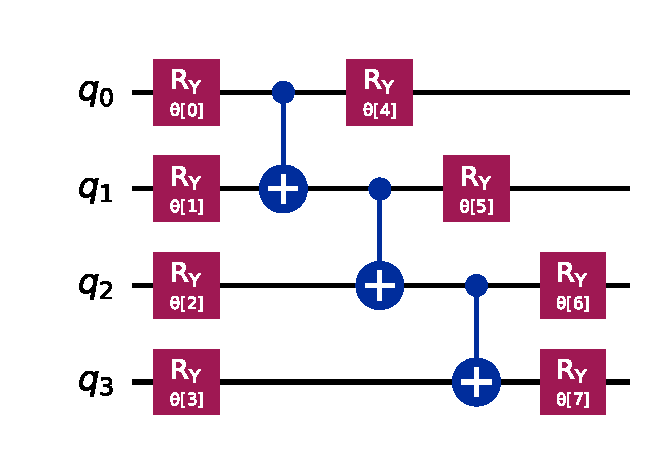
\includegraphics[width=0.8\linewidth]{../plots/block3_02_vqe_ansatz.pdf}
  \caption{The raw VQE ansatz circuit diagram for $L=4$ (reps=1 shown for clarity).}
\end{figure}

\subsection{Ground State Fidelity Validation}
A multi-start optimization loop using the COBYLA algorithm minimizes the energy expectation value.
To ensure the heuristic VQE result is scientifically valid before proceeding to measurements, a strict checkpoint is enforced: the fidelity $F = |\langle\psi_{ED}|\psi_{VQE}\rangle|^2$ must exceed $0.99$. 
Crucially, in the topological phase ($\mu = 0$), the ground state and the first excited state are near-degenerate. The code correctly handles this by summing the overlap probabilities across the degenerate subspace to accurately evaluate the achieved fidelity.

\subsection{Measurement Circuits}
Expectation values are derived via classical post-processing of $8192$ statistical bitstring samples.
For the local Majorana observable $\langle X_0 \rangle$, an $H$ gate is applied to qubit 0 immediately before measurement to switch the basis from $Z$ to $X$.
\begin{figure}[h]
  \centering
  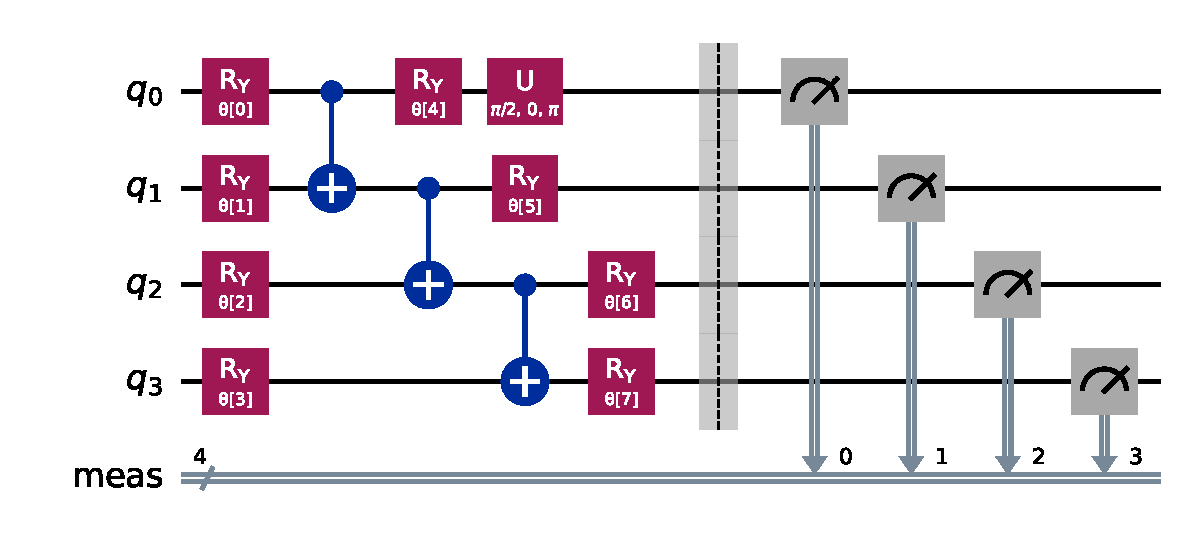
\includegraphics[width=0.8\linewidth]{../plots/block3_03_meas_local.pdf}
  \caption{The measurement circuit for the local observable $\langle X_0 \rangle$.}
\end{figure}

For the non-local string order parameter $\langle Y_{L-1} Z_{L-2} \dots Z_0 \rangle$, the intermediate qubits ($0$ through $L-2$) are measured directly in the $Z$-basis. Qubit $L-1$ undergoes an $S^\dagger$ followed by an $H$ gate to measure in the $Y$-basis.
\begin{figure}[h]
  \centering
  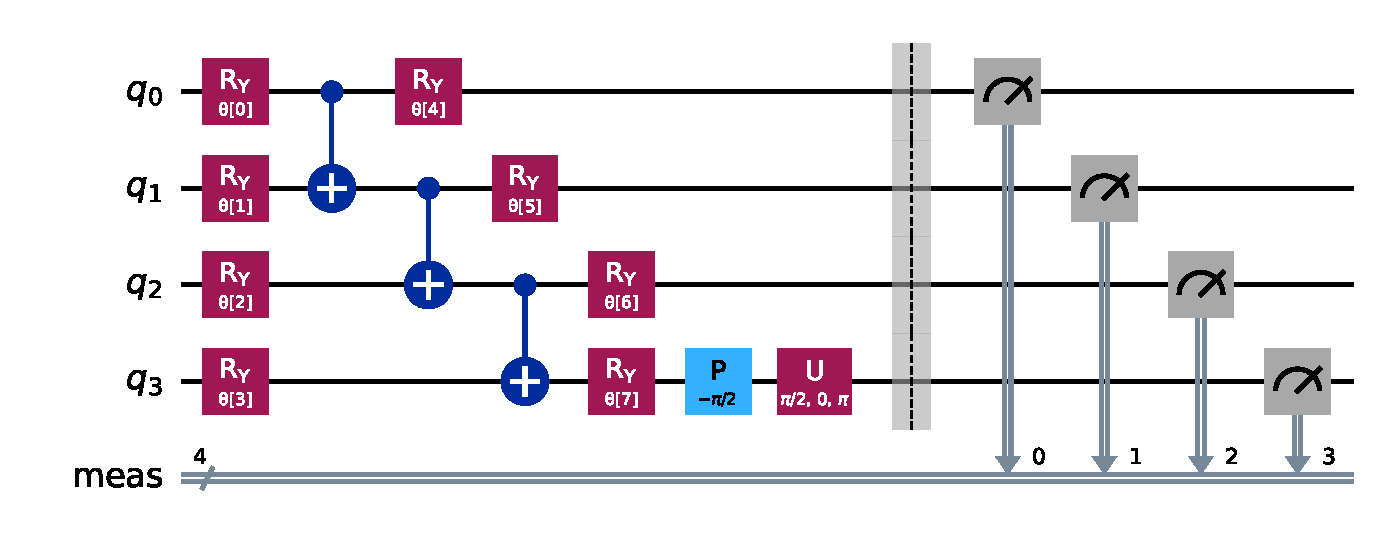
\includegraphics[width=0.8\linewidth]{../plots/block3_04_meas_sop.pdf}
  \caption{The measurement circuit for the non-local String Order Parameter (SOP).}
\end{figure}

\subsection{Results}
Testing this framework at $L=4$ yields successful state preparation with fidelity $\ge 0.998$ across the three representative phases: Topological ($\mu = 0$), Critical ($\mu = 2t$), and Trivial ($\mu = 3t$). The extracted observables confirm the expected behaviors:
\begin{figure}[h]
  \centering
  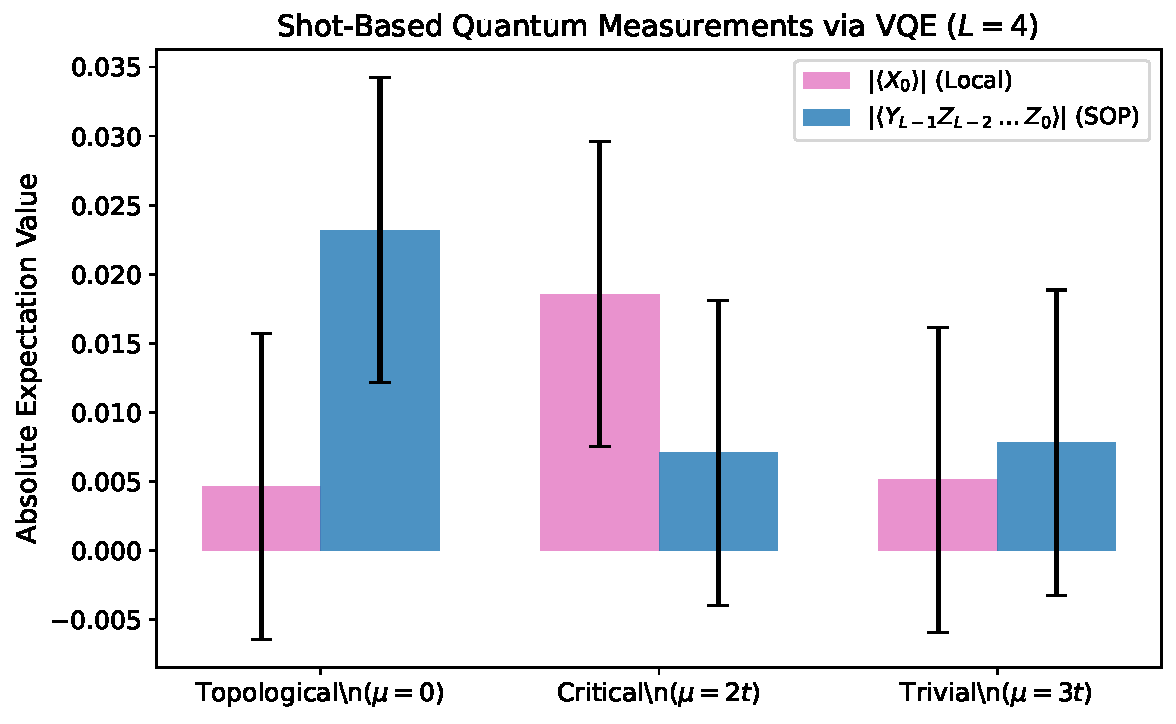
\includegraphics[width=0.7\linewidth]{../plots/block3_01_vqe_observables_test.pdf}
  \caption{Shot-based VQE expectation values at representative phase points.}
\end{figure}

As shown above, the non-local String Order Parameter remains robust in the topological phase but vanishes identically in the trivial phase, serving as a clear, detectable signature of the Kitaev chain's underlying topology on a quantum processor.

\end{document}
